\section{Data and MC Performance}
\label{dataVsMc}
Given the limited number of recorded events passing the trigger and
vertex requirements, the collected statistics allow us to investigate
only the pixel barrel vlolume, that is the tracker region presently
giving the best performance in terms of conversion reconstruction.

A sample of conversions in this region is selected by applying the
following cuts designed to guarantee a good balance between purity and
efficiency:
\begin{itemize}
\item tracks with at least 4 hits;
\item track $d_0\cdot q > 0.1\cm$;
\item track pair opening angle on X-Y plane $\Delta\phi<0.2$;
\item reconstructed conversion vertex radius comprised in the region between $0.8$ and $18\cm$;
\item reconstructed conversion vertex longitudinal position $|z|< 26\cm$;
\item reconstructed transverse momentum of the converted photon $p_T<5\GeV$.
\end{itemize}

Expected performance in terms of efficiency and purity have been
estimated on the MC sample.
Efficiency is defined as the number of associated conversions
$N^{\rm assoc}_{\gamma}$ divided by the total number of simulated
conversions $N^{\rm sim}_{\gamma}$, while purity is defined as
$N^{\rm assoc}_{\gamma}$ divided by the number of reconstructed
conversions $N^{\rm reco}_{\gamma}$.
A reconstructed conversion is considered associated if simulated and reconstructed vertex positions match within a $10\times10\times10\cm^3$ 
box\footnote{A more proper association criteria, based on the hit
  association of the electron tracks, cannot be applied on the used MC
  sample. However, it was proven that the hit and vertex position
  association methods provide compatible results.}.
Figure~\ref{efficpurity} shows that performance degrade for radii greater than $5\cm$, i.e. outside the first pixel barrel layer.
Likely the main reason for this effect is the current tracking configuration where very low $p_T$ tracks can be reconstructed only by using pixel hit triplets as seeds. A different tune of $p_T$ thresholds in iterative tracking steps  could improve performance at larger radii.
%efficiency
%purity
\begin{figure}[!hbtp]
\subfigure[]{
\centering
\label{efficpurity_vs_r}
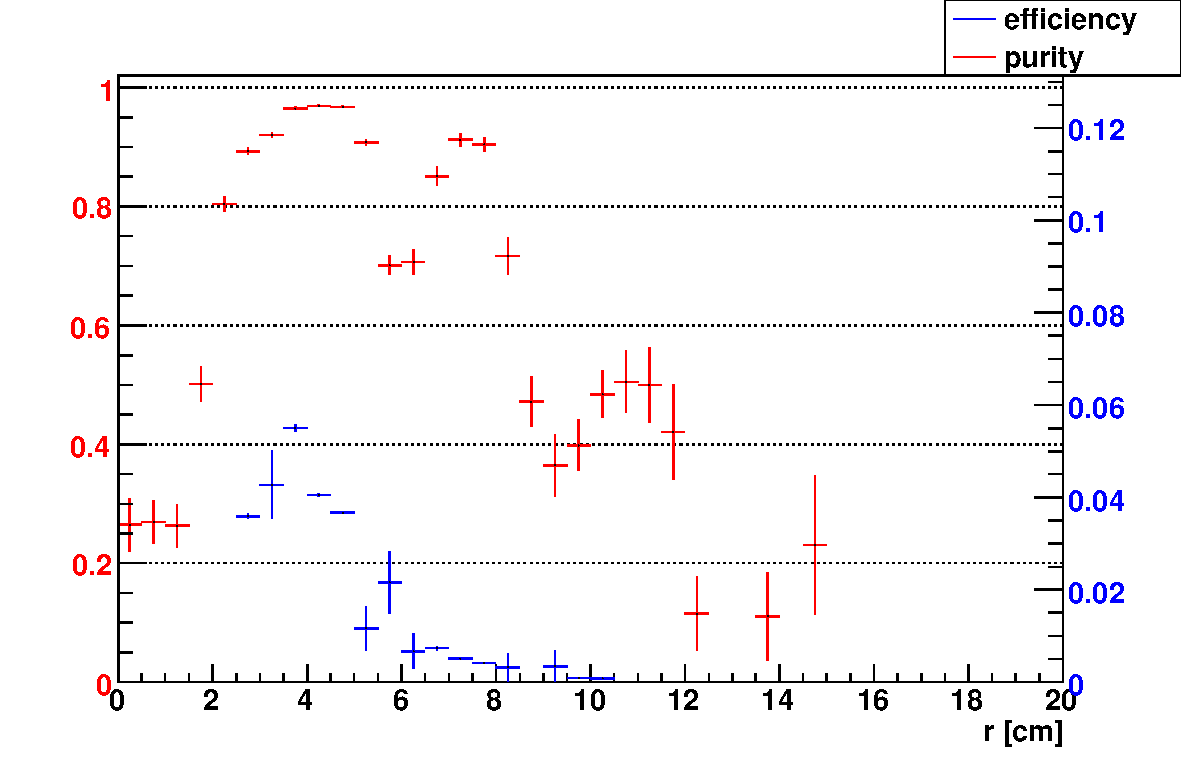
\includegraphics[width=.49\textwidth]{efficpurity_vs_r.pdf}}
\subfigure[]{
\centering
\label{efficpurity_vs_pt}
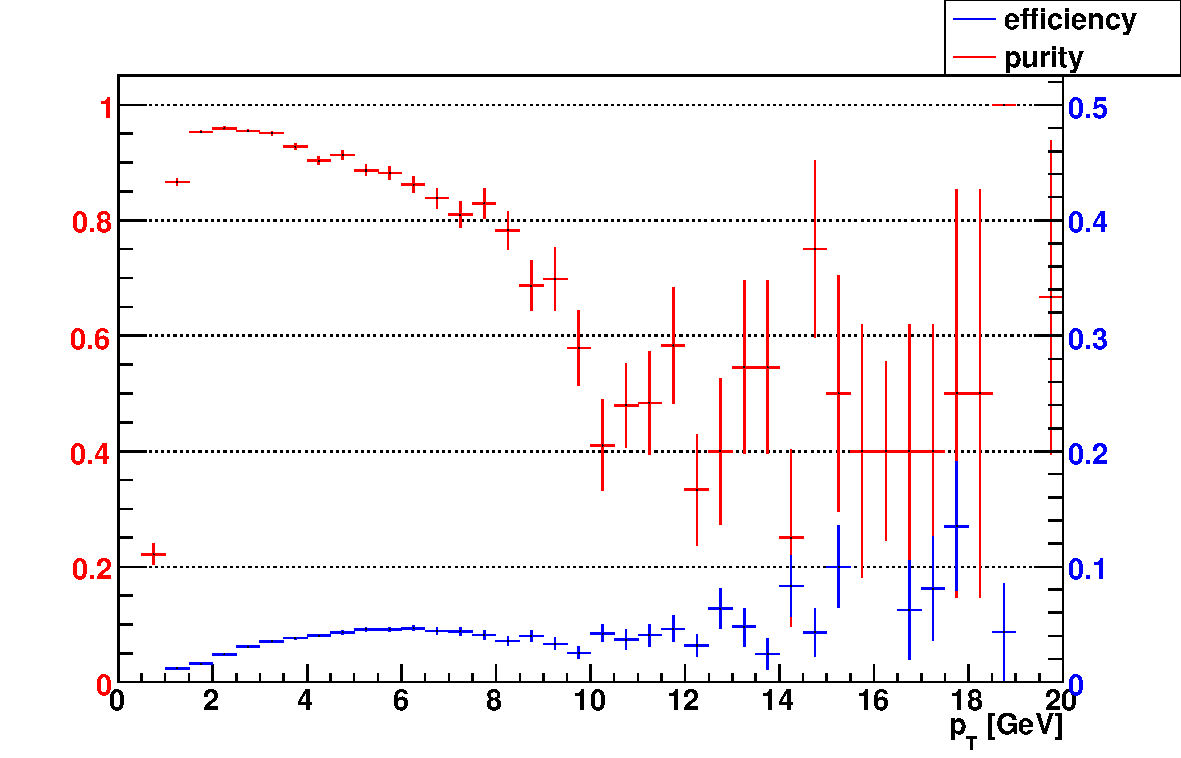
\includegraphics[width=.49\textwidth]{efficpurity_vs_pt.pdf}}
\caption{Efficiency (blue) and purity (red) of the Tracker-only conversion finding algorithm: \subref{efficpurity_vs_r} as a function of $r$; \subref{efficpurity_vs_pt} as a function of $p_T$.}
\label{efficpurity}
\end{figure}

Data versus Monte Carlo simulation comparison has been done on some basic distributions to check the conversion finding algorithm performances with first collision data. The distributions of the reconstructed transverse momentum ($p^{\gamma}_T$) and of the pseudo-rapidity ($\eta^\gamma$) of the converted photon are shown in Fig. ~\ref{fig:pt} and Fig.~\ref{fig:eta}, respectively. The radius of the conversion vertex ($r$) distribution is shown in Fig.~\ref{fig:r}. 

All distributions, given either in linear and in logarithmic scale, result in a pretty good agreement between data and Monte Carlo as far as the shapes are concerned. The overall number of conversions candidates is $\sim10\%$ higher in data with respect to the Monte Carlo simulation. Such small discrepancy is acceptable for the sake of the present preliminary study. It could be due, among several effects, to differences between data and simulation in the number of fakes or at the level of the photon flux.
\begin{figure}[!hbtp]
\centering
\subfigure[]{
\label{subfig:pt_lin}
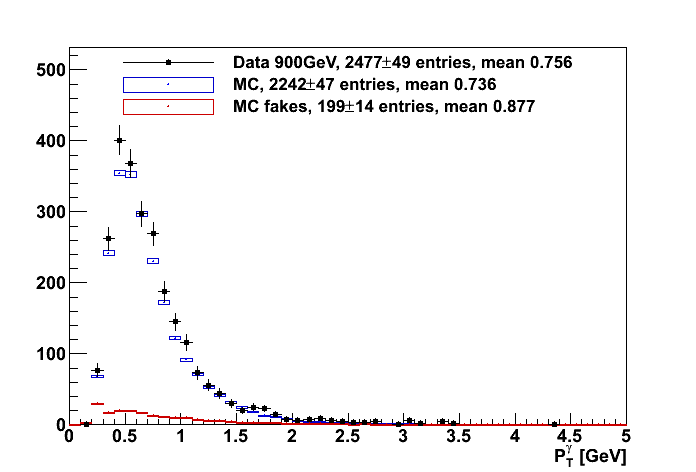
\includegraphics[width=.49\textwidth]{pt_lin.png}}
\subfigure[]{
\label{subfig:pt_log}
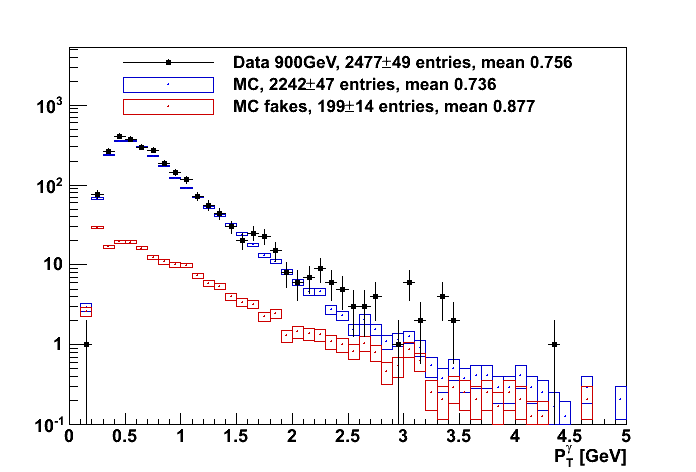
\includegraphics[width=.49\textwidth]{pt_log.png}}
\caption{Distribution of the reconstructed tranverse momentum ($p^{\gamma}_T$) of the converted photon in linear~\subref{subfig:pt_lin} and logarithmic~\subref{subfig:pt_log} scale. Data is shown in black dots and Monte Carlo  simulation in blue boxes. Red boxes represent the estimated fake contribution.}
\label{fig:pt}
\end{figure}

\begin{figure}[!hbtp]
\centering
\subfigure[]{
\label{subfig:eta_lin}
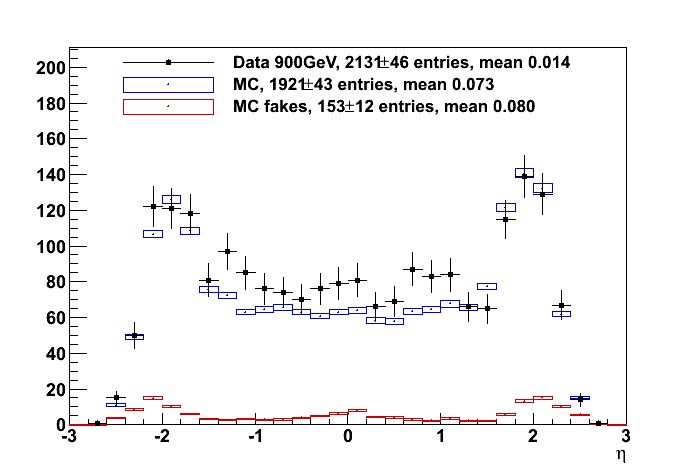
\includegraphics[width=.49\textwidth]{eta_lin.png}}
\subfigure[]{
\label{subfig:eta_log}
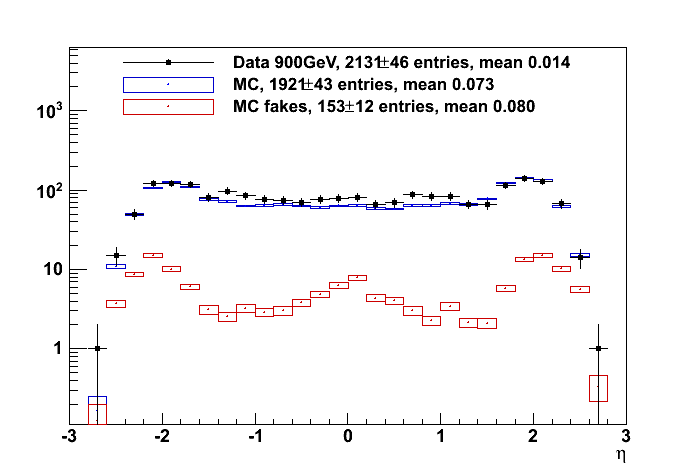
\includegraphics[width=.49\textwidth]{eta_log.png}}
\caption{Distribution of the reconstructed pseudorapidity ($\eta^\gamma$) of the converted photon in linear~\subref{subfig:eta_lin} and logarithmic~\subref{subfig:eta_log} scale. Data is shown in black dots and Monte Carlo  simulation in blue boxes. Red boxes represent the estimated fake contribution.}
\label{fig:eta}
\end{figure}

\begin{figure}[!hbtp]
\centering
\subfigure[]{
\label{subfig:r_lin}
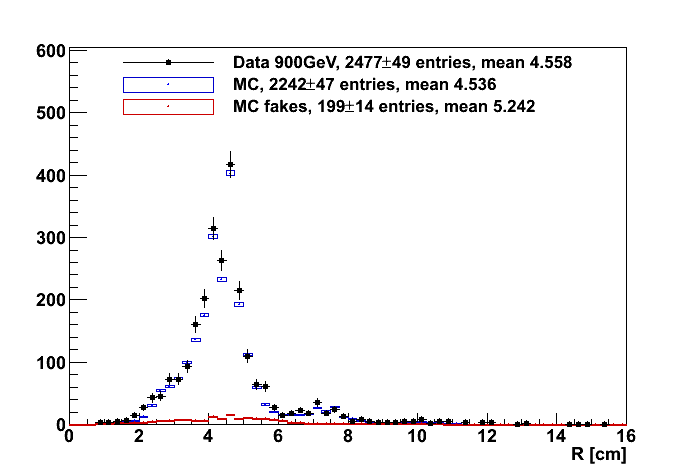
\includegraphics[width=.49\textwidth]{r_lin.png}}
\subfigure[]{
\label{subfig:r_log}
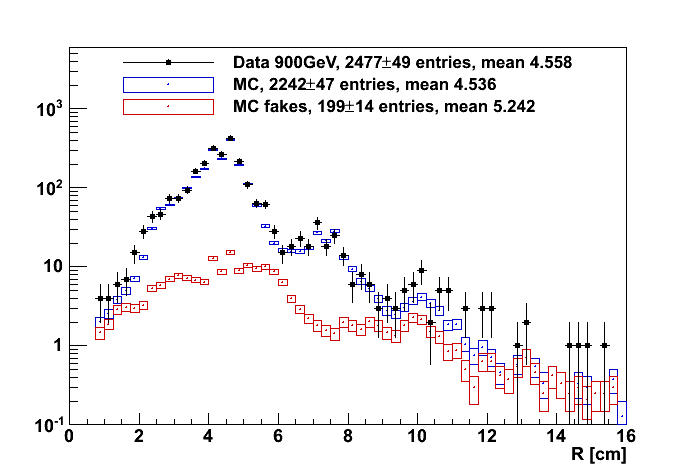
\includegraphics[width=.49\textwidth]{r_log.png}}
\caption{Distribution of the reconstructed conversion radius ($r$) in linear~\subref{subfig:r_lin} and logarithmic~\subref{subfig:r_log} scale. Data is shown in black dots and Monte Carlo simulation in blue boxes. Red boxes represent the estimated fake contribution.}
\label{fig:r}
\end{figure}
